% This is LLNCS.DEM the demonstration file of
% the LaTeX macro package from Springer-Verlag
% for Lecture Notes in Computer Science,
% version 2.4 for LaTeX2e as of 16. April 2010
%
\documentclass[10pt]{llncs}
\usepackage{xeCJK}
\usepackage{amsmath}
\usepackage{listings}
\usepackage{amssymb}
\usepackage{float}
\usepackage{graphicx}
%
\usepackage{makeidx}  % allows for indexgeneration
%
\begin{document}
    \title{Report: Show/prove how "always" and "until" can be derived from "Weak Until"}
    \author{林奇峰, Qifeng Lin\\Student ID:17214656}
    \date{\today}
    \institute{SYSU}
    \maketitle

    \begin{question}
         show how "always" and "until" can be derived from "Weak Until".
        \begin{align*}
          \Box\varphi &\equiv \varphi\textbf{W}\text{false} \\
          \varphi\textbf{U}\psi & \equiv(\varphi\textbf{W}\psi)\wedge\diamond\psi\\
          \varphi\textbf{W}\psi &\equiv( \varphi\textbf{U}\psi)\vee\diamond\phi
        \end{align*}
    \end{question}
    Here, we replace $\varphi$ and $\psi$ with "a" and "b".
    \begin{definition}
        $\sigma,i\models\textbf{F}\phi \text{ iff there exists j such that }i\leq j\leq|\sigma| \text{ and } \sigma,j\models\phi$
    \end{definition}
    The definition above can be showed as Fig1.
    \begin{figure}[H]
      \centering
      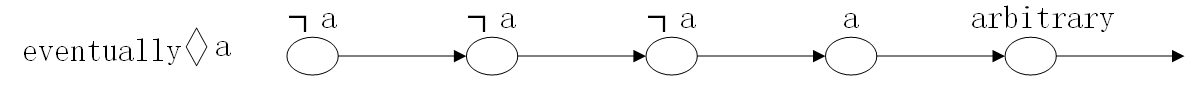
\includegraphics[width=5.0in,height=0.3in]{7.png}
      \caption{"eventually $\diamond$a"}
    \end{figure}

    \begin{definition}
        $sigma,i\models\textbf{G}\phi \text{ iff for all j such that }i\leq j\leq|\sigma|, \text{ we have } \sigma,j\models\phi$
    \end{definition}
    The definition above can be showed as Fig2. We can see that "always" means that a property is always true and "until", "a {\textbf U} b", means that a is always true until b is true.
    \begin{figure}[H]
      \centering
      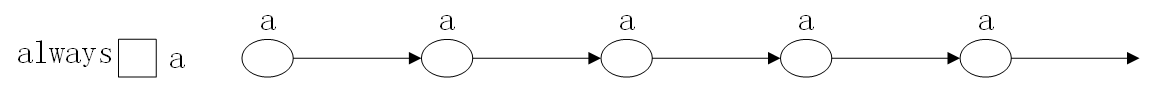
\includegraphics[width=5.0in,height=0.3in]{3.png}
      \caption{"always"}
    \end{figure}
    \begin{definition}
    $\sigma,i\models\phi\textbf{U}\psi \text{ iff there exists j, }i\leq j\leq|\sigma| \text{ such that }\sigma,j\models\psi\text{, and for all k such that }i\leq k\leq|\sigma|,\text{ we have }\sigma,k\models\phi$
    \end{definition}
    The definition above can be showed as Fig3.
    \begin{figure}[H]
      \centering
      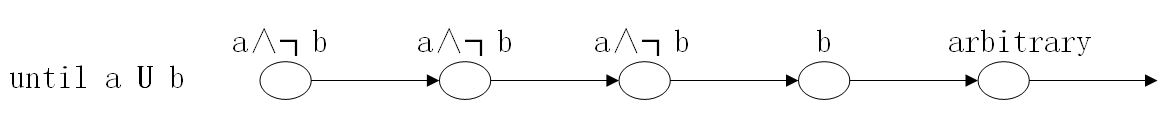
\includegraphics[width=5.0in,height=0.4in]{1.png}
      \caption{"until"}
    \end{figure}


    From $\varphi\textbf{W}\psi\equiv( \varphi\textbf{U}\psi)\vee\diamond\phi$, we can obtain Fig4. We can see that "weak until", "a \textbf{W} b" can be divided into two cases: one is with b and the other one is without b.
    Therefore, for "a \textbf{W} false", we can obtain Fig5.
    \begin{figure}[H]
      \centering
      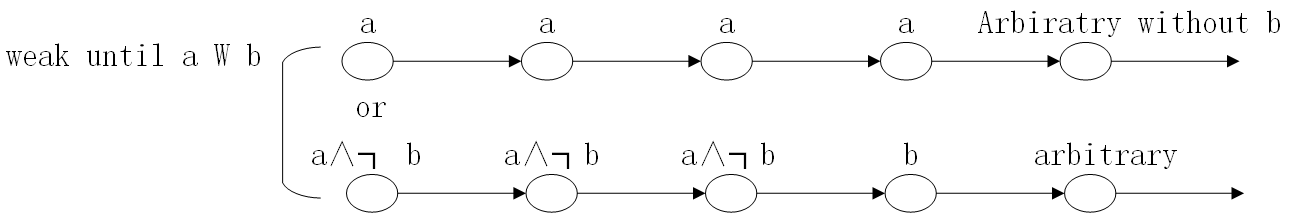
\includegraphics[width=5.0in,height=0.6in]{4.png}
      \caption{"weak until"}
    \end{figure}
    \begin{figure}[H]
      \centering
      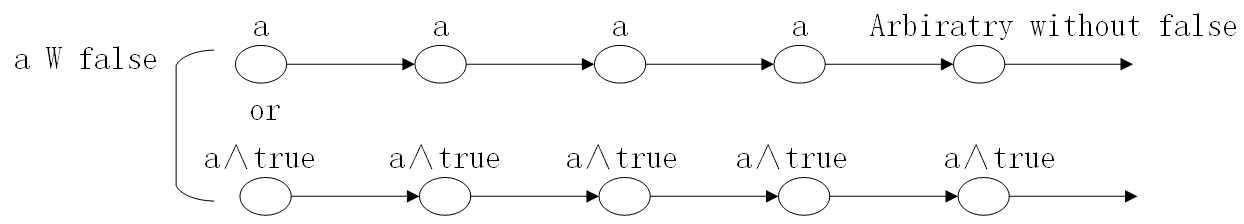
\includegraphics[width=5.0in,height=0.6in]{5.png}
      \caption{"a \textbf{W} false"}
    \end{figure}
      We need to explain how to acquire Fig5. Firstly, for the first case, we can see that "a" is always true because "false" does't happen. And for the second case, since the negation of "false" is "true" and "false" means that it never occurs, it can be reasoned that "a $\wedge$ true" is always true. But "a $\wedge$ true" is equivalent to "a". Therefore, "$\Box$a" is equivalent to "a \textbf{W} false". That is, $\Box\varphi\equiv \varphi\textbf{W}\text{false}$.

       As for "(a \textbf{W} b)$\wedge\diamond$b", since "$\diamond$b" guarantees the occurrence of b, the first case of "(a \textbf{W} b)" is excluded and the second case remains. The second case is the form of "a \textbf{W} b". Therefore, $\varphi\textbf{U}\psi \equiv (\varphi\textbf{W}\psi)\wedge\diamond\psi$. It can be show as Fig6.
    \begin{figure}[H]
      \centering
      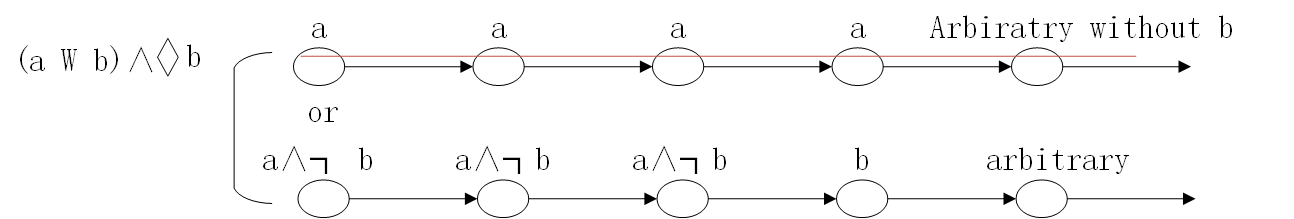
\includegraphics[width=5.0in,height=0.6in]{6.png}
      \caption{"(a \textbf{W} b)$\wedge\diamond$b"}
    \end{figure}

    \begin{equation}\label{8.31}
                  \begin{split}
                     \overline{A}(h|\vec{x}) & =\sum_{i=1}^{T}w_iE(h_i|\vec{x})-E(H|\vec{x}) \\
                       & =\overline{E}(h|\vec{x})-E(H|\vec{x})
                  \end{split}
                \end{equation}

\end{document}
